% This document must be compiled with LuaLaTeX
\documentclass[12pt,article]{memoir}

\usepackage[letterpaper, portrait, margin=1in]{geometry}	% Standard page setup
\usepackage[USenglish]{babel}								% English typsetting conventions
\usepackage{fancyhdr}										% Headers and footers
\usepackage{graphicx}										% Additional graphics options
\usepackage{xcolor}											% Better colors
\usepackage{xpatch}											% Better macro patches
\usepackage{hyperref}										% Hyperlinks
\usepackage{fontspec}										% Custom fonts
\usepackage{tikz}											% Graphics creation
\usepackage{float}											% Figure positioning
\usepackage{tabu}											% Better tables
\usepackage[style=ieee, backend=biber]{biblatex}			% Bibliography
\usepackage[font={small,it}]{caption}						% Italic captions
\setsansfont{NeueHaasUnicaPro}
\usetikzlibrary{calc}
\usepackage[yyyymmdd]{datetime} % change date format to yyyy/mm/dd to fit ISO8601

\renewcommand{\familydefault}{\sfdefault} % set font
\renewcommand{\dateseparator}{--} % change date-seperators to - to fit ISO8601

\renewcommand\contentsname{Table of Contents}

\chapterstyle{section}
\renewcommand*{\chapnumfont}{\normalfont\HUGE\bfseries\sffamily}
\renewcommand*{\chaptitlefont}{\normalfont\HUGE\bfseries\sffamily}

\makeatletter 
% define macro for itemcode
\newcommand\itemcode[1]{\renewcommand\@itemcode{#1}}
\newcommand\@itemcode{}

% define macro for rev number
\newcommand\revnumber[1]{\renewcommand\@revnumber{#1}}
\newcommand\@revnumber{}
\makeatother

\definecolor{orbitOrange}{RGB}{250,62,0} % the ORBiT orange

\setlrmarginsandblock{2.5cm}{2.5cm}{*}
\setulmarginsandblock{2.5cm}{*}{1}
\checkandfixthelayout 

\setlength{\beforechapskip}{0cm} % reduce chapter spacing

\hypersetup{
    colorlinks,
    citecolor=black,
    filecolor=black,
    linkcolor=black,
    urlcolor=black
}

% Background swoosh
\newcommand\OrbitBackground[1]{% For a logo drawn with TikZ
	\begin{tikzpicture}[remember picture,overlay] % draw background
	\coordinate (bl) at (current page.south west);
	\coordinate (r) at (current page.east);
	\coordinate (A) at ($(bl)+(0,3cm)$);
	\coordinate (B) at ($(r)+(0,-2cm)$);
	\coordinate (C) at (current page.south east);
	\coordinate (ctrlNode) at ($(current page.south) + (0cm,1cm)$);
	\coordinate (ctrlNode2) at ($(current page.south east) + (-1cm,1cm)$);
	\fill[orbitOrange, fill opacity={#1}]
	(A) .. controls (ctrlNode) and (ctrlNode2) .. (B) -- (C) -- (bl);
	\node [white] at ($(C) + (-3cm,1cm)$) {2015-\the\year \ ORBiT@SU};
	\end{tikzpicture}
}
% Bibliography database
\addbibresource{DR00002.bib}
%**********************************************************************
%Document titles etc. defined here: (replace [] as well)
\title{OA-II VEH Camera System Design}
\author{Jinzhi Cai}
\itemcode{DR00002}
\revnumber{A04}
\date{\today}
%end of document titles etc.
%**********************************************************************

% set header style
\makeatletter
\pagestyle{fancy}
{
	\fancyheadoffset{0cm}

	\lhead{\@title \ - \@itemcode}
	\rhead{Page: \thepage }
	%\chead{\leftmark} % section name
}
\makeatother

\cfoot{\OrbitBackground{0.2}}

\begin{document}
	
\OrbitBackground{1}

\makeatletter

\includegraphics[width=\textwidth]{../Templates/logo.jpg}\\[4ex]
\begin{center}
	\bfseries \fontsize{50}{50}\selectfont  \@title \\[2ex]
	\LARGE  \@itemcode
\end{center}
\vfill
\begin{flushright}
	\LARGE Rev: \@revnumber\\
	\large \@author\\
	\large \@date\\[18ex]
\end{flushright}
\makeatother
\thispagestyle{empty}
\newpage

\tableofcontents*
\thispagestyle{fancy}
\newpage

\tableofcontents*
\clearpage
%**********************************************************************
% Everything after this is the main document. Edit below this line,

\chapter{Introduction}
\section{Scope}
This document discusses current camera technology and outlines a design that will fulfill the needs for OA-II VEH.
\section{Purpose}
The goal for this document is to come up with a design that will provide four 1080p 60Hz video steams and store that data to a central storage media by researching current options in camera technology.
\section{Revision History}

\begin{table}[H]
	\centering
	\begin{tabu}{r || c | c | c }
		Rev\# & Editor & Delta & Date\\ \hline
		A01 & Jinzhi Cai & Initialize & 2019-7-13\\ \hline
		A02 & Jinzhi Cai & Add detail & 2019-7-15\\
		A03 & Jinzhi Cai & Add Jetson Nano & 2019-7-24\\
		A04 & Gabriel Smolnycki & Minor grammar edits & 2019-08-26
	\end{tabu}
	\caption{Summary of Revision History}
	\label{tab:rev}
\end{table}

\newpage
\chapter{General Structure of Camera System}
\section{Introduction}
The most basic camera system has three parts. The camera sensor is the device that will receive data from the environment and transfer it via the camera interface. The data that flows out from the sensor is called raw data. It contains all the information that the camera takes in from the sensor. A 1080p 60Hz camera has $1920*1080=2073600 pixels$, and one pixel usually take $3 Bytes$ to save. For each second, $2073600*3*60=373248000Bytes$ will be created. That will be $355.96MB/s$ for one single camera. An encoder is used to compress the video steam smaller for it to be transmitted via long distance data link(usually with in $1MB/s$).\cite{zhidao:Video} The storage unit is then used to save the video steam to a file for future replay.
\begin{figure}[htp]
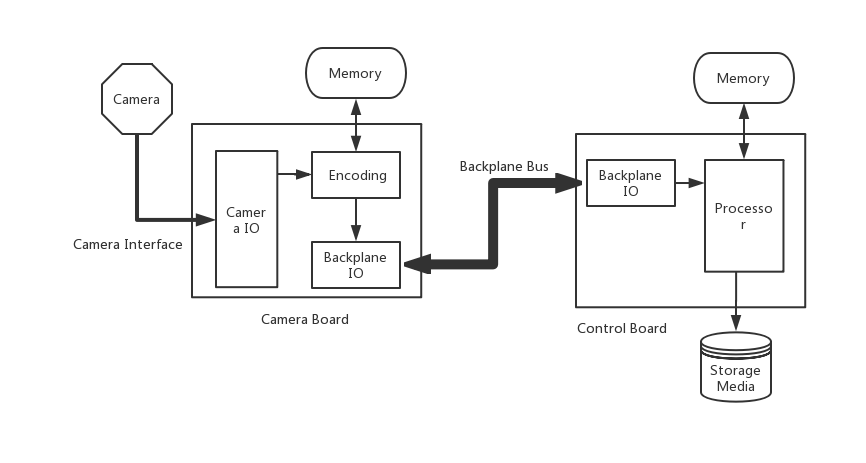
\includegraphics[width=\textwidth]{img/DR00002_GenDia.png}
 \caption{General Structure of Camera System}	
\end{figure}
\newpage
%
%**********************************************************************
\chapter{Camera Sensor and Relative Interface}
\section{Introduction}
The sensor is the most important part of the system. Using a classical implementation, in the same way as a monitor would, data is output as video signal to an external device. For each pixel clock, data of a pixel has been transmitted. After few clock(depend on the resolution), Line Sync rise to indicate one line data is finish transmission. The Frame Sync is indicate a frame of pixel data is sent. However, modern camera sensor usually use one of those three camera interface. Some of the is similar with the classic one, and other improve it.
\begin{figure}[htp]
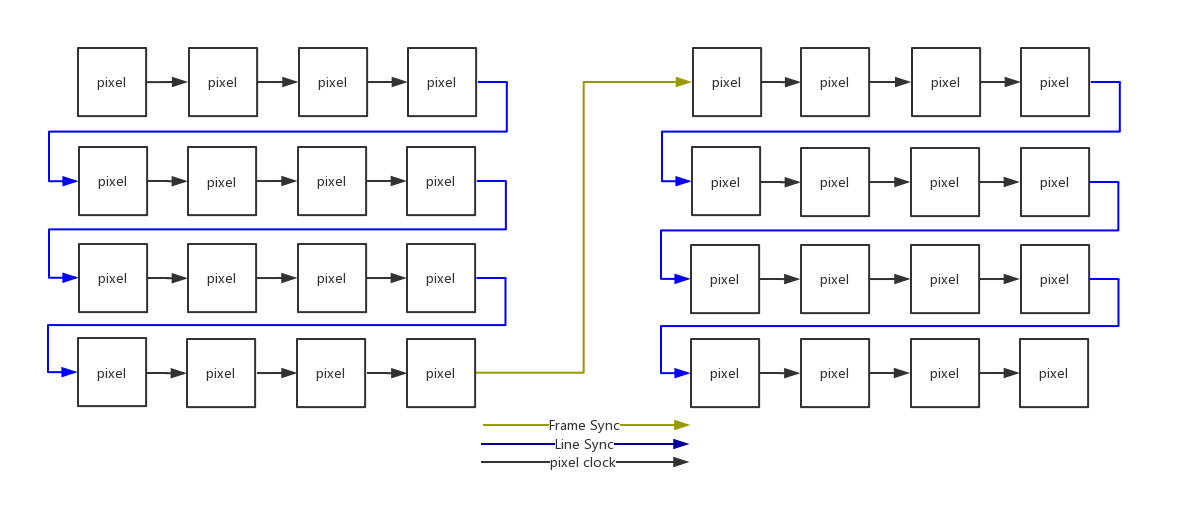
\includegraphics[width=\textwidth]{img/DR00002_Cam.png}
 \caption{Classic Video Stream}	
\end{figure}
\newpage
\section{DVP Interface} 
The DVP interface is use the classic video interface to transmit data out from the sensor. The I2C bus(SCK, SDA) that inside the interface is use to configure the camera. The main clock is use to provide a clock for the camera. The VSYNC, HSYNC, PCLK is the clock system that help processor to indicate the weight and height of frame. The D OUT is data that coming out from the camera. It have low requirement on the trace and sample interface design. However, it can not offer long distance transmission and high speed clock. It usually use at low end 240p camera.\cite{blog:DVP}
\begin{figure}[htp]
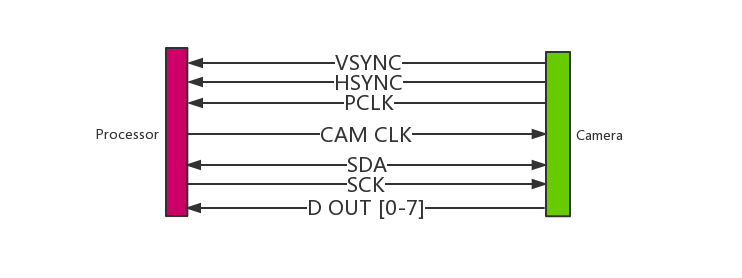
\includegraphics[width=\textwidth]{img/DR00002_DVP.png}
 \caption{Physical Layer for DVP Interface}	
\end{figure}
\begin{description}
	\item[\textbf{D OUT}]Data out put
	\item[\textbf{VSYNC}]Lane Sync Signal
	\item[\textbf{HSYNC}]Frame Sync Signal
	\item[\textbf{PCLK}]Pixel Clock
	\item[\textbf{CAM CLK}]Main Camera Clock
	\item[\textbf{SDA}]I2C Data Line
	\item[\textbf{SCK}]I2C Clock Line
\end{description}
\newpage
\section{LVDS Interface}
The LVDS camera interface is use LVDS technology to improve classic DVP interface. It use differential signal to transmitting data. It increase the lane it need to send data, but differential signal can prevent common mode interference which limit the DVP clock for increasing.\cite{blog:LVDS}
\begin{figure}[htp]
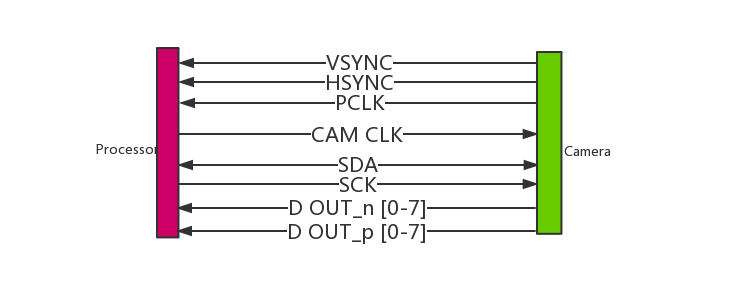
\includegraphics[width=\textwidth]{img/DR00002_LVDS.png}
 \caption{Physical Layer for LVDS Interface}	
\end{figure}
\begin{description}
	\item[\textbf{DOUT n/p}]Differential Data Lane
	\item[\textbf{VSYNC}]Lane Sync Signal
	\item[\textbf{HSYNC}]Frame Sync Signal
	\item[\textbf{PCLK}]Pixel Clock
	\item[\textbf{CAM CLK}]Main Camera Clock
	\item[\textbf{SDA}]I2C Data Line
	\item[\textbf{SCK}]I2C Clock Line
\end{description}
\newpage
\section{MIPI CSI-2 Interface}
The MIPI CSI-2 camera interface$\footnote{Might only available in high-end chip.}$ is different from the old one. The goal for this bus is to cut down the lane count for camera module and allow more data flow to the processor. In structure, the MIPI CSI-2 camera interface use different way to communicate. The MIPI interface use package as the data communication unit. Inside the sensor, data will be pack into a package and send it via the two or four data lane. The same process will reverse and output the raw camera data. MIPI camera will allow 1080p 60Hz or 4K 30Hz.\cite{blog:MIPICSI2}
\begin{figure}[htp]
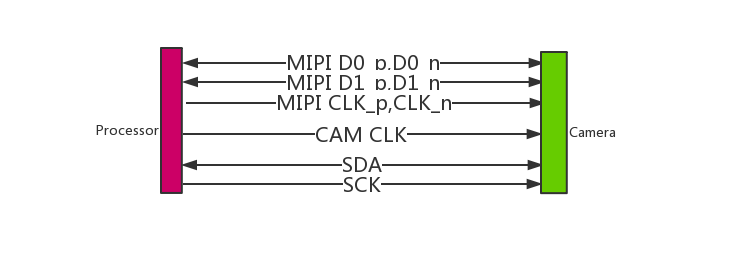
\includegraphics[width=\textwidth]{img/DR00002_MIPI.png}
 \caption{Physical Layer for 2 Lane MIPI Interface}	
\end{figure}
\begin{description}
	\item[\textbf{MIPI D0n/p}]MIPI Data Lane 0
	\item[\textbf{MIPI D1n/p}]MIPI Data Lane 1
	\item[\textbf{MIPI CLKn/p}]MIPI Clock
	\item[\textbf{CAM CLK}]Main Camera Clock
	\item[\textbf{SDA}]I2C Data Line
	\item[\textbf{SCK}]I2C Clock Line
\end{description}
\section{USB Interface (UVC)}
The USB camera interface$\footnote{It do have success example by using ZYNQ SoC FPGA.}$ is different with the rest of the interface. In those camera, it include DSP chip that already finish the video compression.\cite{blog:USB} It is easy to use and support 60fps.$\footnote{With High End SoC chip}$
\newpage
%**********************************************************************
\chapter{Camera Interface Bridge Chip}
\section{Lattice CrossLink}
The CrossLink is Lattice made small scale MIPI bridge FPGA.$\footnote{Too small for hardware encoder}$ It include two MIPI D-PHY and up to 8 MIPI data lane. It also support interface translation (MIPI CSI-2 -> DVP).\cite{Lattice:CrossLink}
\begin{figure}[htp]
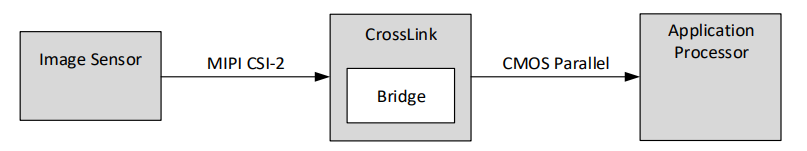
\includegraphics[width=\textwidth]{img/DR00002_CrossLink.png}
 \caption{Block Diagram for CrossLink}	
\end{figure}
\section{Toshiba Camera Interface Bridge}
The Toshiba Camera Interface Bridge is a stand alone chip that can converse MIPI CSI-2 bus to DVP bus. It also offer I2C bus to configure chip setting.\cite{toshiba:InterfaceBridge}
\begin{figure}[h]
\begin{center}
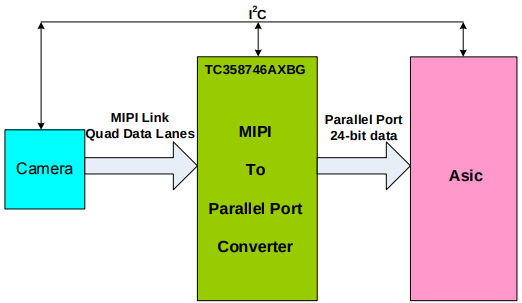
\includegraphics[width=0.7\textwidth]{img/DR00002_Toshiba.png}
 \caption{Block Diagram for Toshiba}	
 \end{center}
\end{figure}
\newpage
%**********************************************************************
\chapter{H.264 Video Steam Encoding}
\section{Introduction}
The H.264 Encoder is another important unit in the camera system. Due to the data flow of a camera sensor is too much for the backplane bus, compression is necessary.
\section{IP Core Description}
\subsection{SoC Technology}
This IP core fit for both \textbf{Intel} and \textbf{Xilinx} \cite{ipcore:SoCTech} \cite{ipcore:A2ETech}.
\begin{table}[H]
	\centering
		\begin{tabu}{r || c | c | c }
		Version & LUT use & Test Platform & Price for Platform\\ \hline
		Standard Version & 110k & Zynq-7 Z7045 & \$1000\\
		Slim Version & 50k & Artix-7 XC7A200T & \$300\\
		I-Frame Version & 45k & Spartan-6 LX150 & \$200\\
		\end{tabu}
	\caption{Encoder Summary}
	\label{tab:encoders}
\end{table}
\subsection{A2E Technology}
\begin{table}[H]
	\centering
		\begin{tabu}{r || c | c | c }
		Version & LUT use & Test Platform & Price for Platform\\ \hline
		Xilinx(1080p 30Hz) & 11K & Zynq-7 Z7020 & \$300\\
		Xilinx(1080p 60Hz) & 11K & Kintex-7 & \$500\\
		Xilinx(1080p 180Hz) & 11K & Zynq UltraScale & \$1000\\\hline
		Intel(1080p 30Hz) & 8K & Cyclone V SoC & \$500\\
		\end{tabu}
	\caption{SoC Summary}
	\label{tab:socs}
\end{table}
\newpage
\section{Encoding SoC Chip}
\subsection{HiSilicon Hi3559}
Hi3559 is HiSilicon made new generation mobile camera soc. It support MIPI interface and H.264 Video encoding up to 1080P 60Hz. It can output video via USB 2.0 bus.\cite{huawei:Hi3559}
\begin{figure}[htp]
\begin{center}
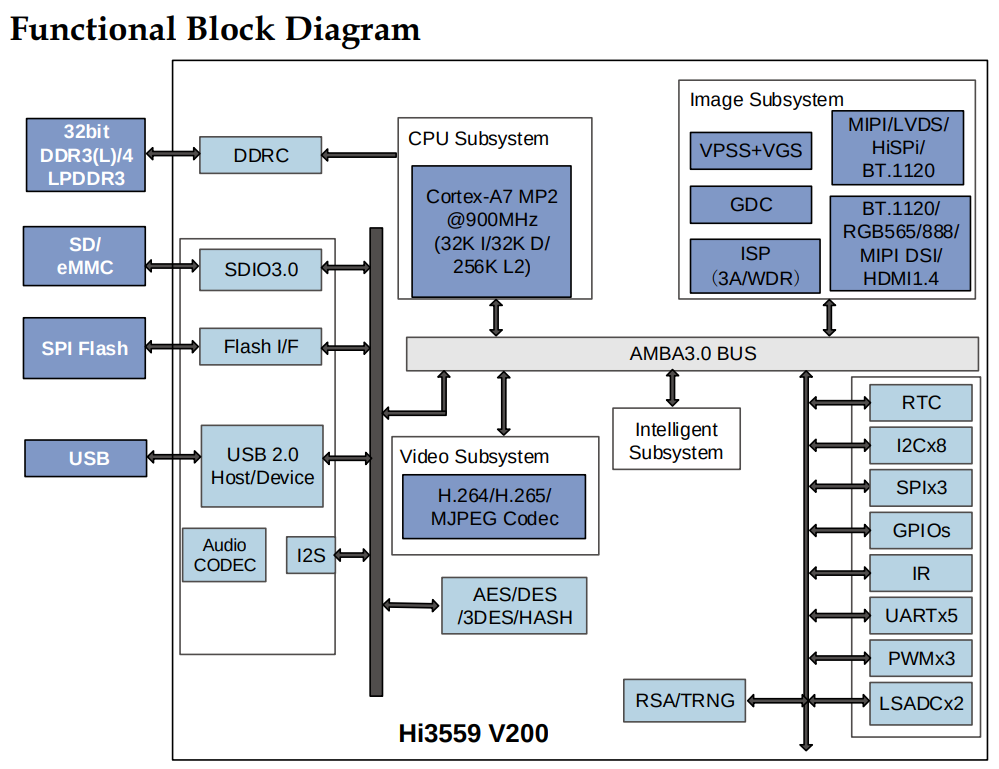
\includegraphics[width=\textwidth]{img/DR00002_Hi3559.png}
 \caption{Block Diagram for Hi3559}	
\end{center}
\end{figure}
\newpage
\subsection{OmniVision OV798}
OV798 is OmniVision made camera soc. It support MIPI interface and H.264 Video encoding up to 720P 60Hz. It can output video via USB 2.0 bus.\cite{omni:OV798}
\begin{figure}[htp]
\begin{center}
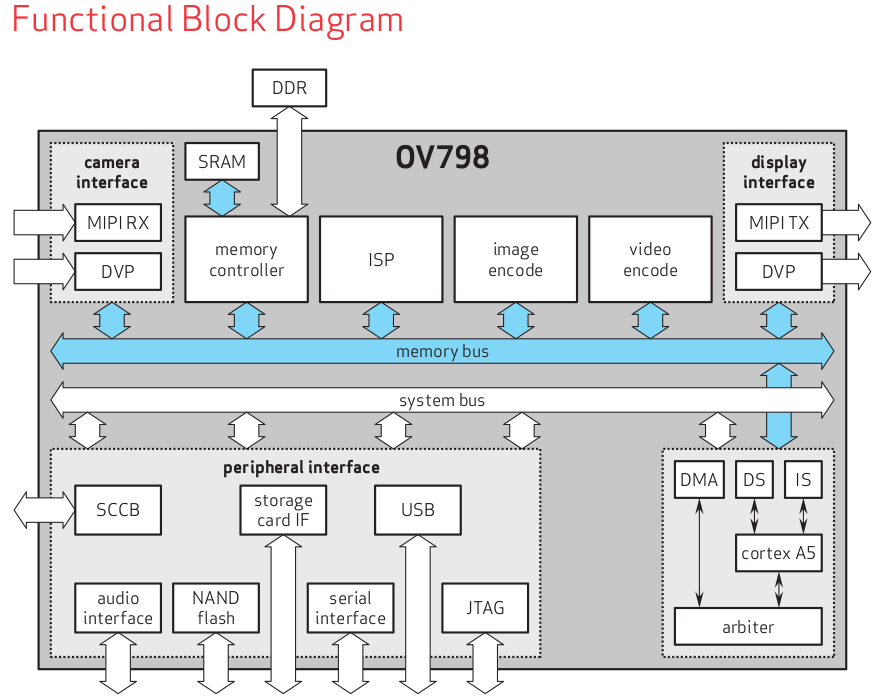
\includegraphics[width=\textwidth]{img/DR00002_Omni.png}
 \caption{Block Diagram for OV798}	
\end{center}
\end{figure}
\newpage
\subsection{Ambarella H22}
The Ambarella H22 SoC for consumer applications is a system-on-chip that integrates an advanced image sensor pipeline (ISP), H.265 (HEVC) and H.264 (AVC) encoders , and a powerful Quad core ARM® Cortex™-A53 CPU.\cite{ambarella:H22}$\footnote{H22 Video SoC for Consumer Applications}$
\begin{figure}[htp]
\begin{center}
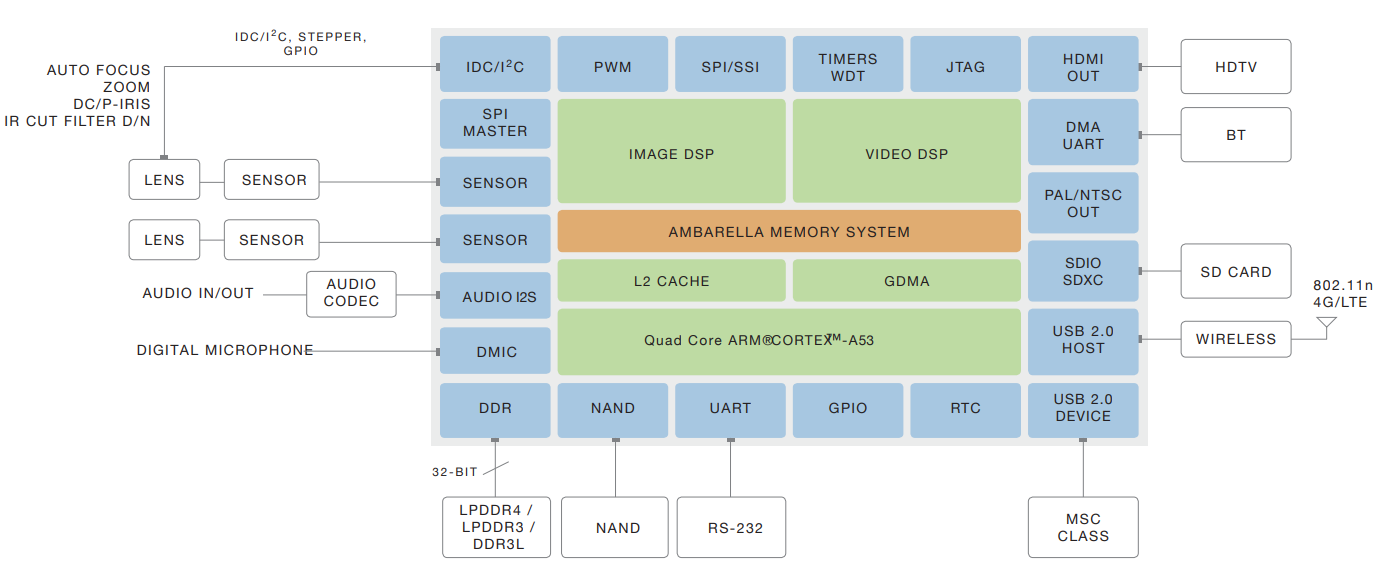
\includegraphics[width=\textwidth]{img/DR00002_Ambarella.png}
 \caption{Block Diagram for Ambarella H22}	
\end{center}
\end{figure}

\newpage
\section{DSP Chip}
\subsection{TMS320C6678 DSP}
The TMS320C6678 DSP is a highest-performance fixed/floating-point DSP that is based on TI's KeyStone multicore
architecture. Incorporating the new and innovative C66x DSP core, this device can run at a core speed of up to
1.4 GHz.\cite{ti:TMS320C6678}$\footnote{TMS320C6678 Multicore Fixed and Floating-Point Digital Signal Processor}$
\begin{figure}[htp]
\begin{center}
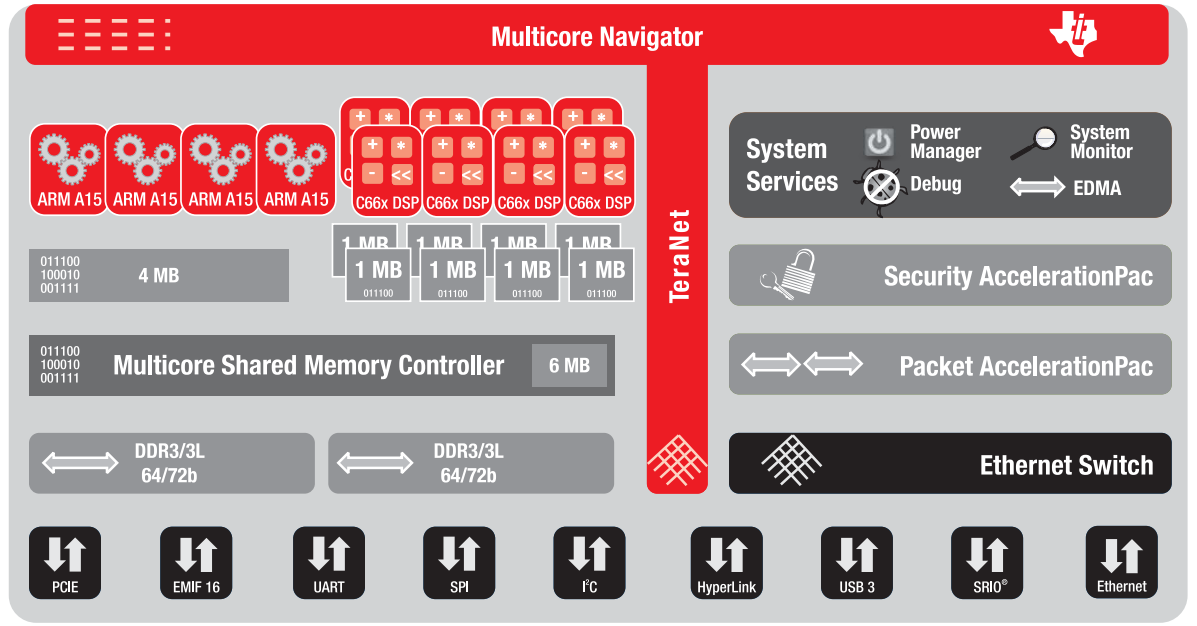
\includegraphics[width=\textwidth]{img/DR00002_DSP.png}
 \caption{Block Diagram for Ambarella H22}	
\end{center}
\end{figure}
\newpage
\section{GPU Module}
\subsection{Jetson Nano}
The Jetson Nano is a GPU computing module what NVIDIA produce for GPU AI computer. It come with 6 MIPI CSI-2 interface and able to handle about 4K 60fps encoding. In the output option, it support PCIe output which can use as the interface. The only problem is it will require extra thermal solution due to the heat it produce and FPGA adoption program to translate the data to backplane bus.\cite{nv:JetsonNano}

\newpage

\chapter{System Diagram}
\section{USB camera with SoC FPGA chip}
This plan will use USB 2.0 UVC interface to connect one camera to a SoC FPGA chip. The chip will translate the data to back-plane bus and send to the storage device. It can use the builtin USB controller and system driver, which reduce the development time. It could up grade to better camera set by using self developed module. But the builtin USB interface will limited the bit-rate encoding use and might cause blur when the sensor meet frequently vibration.
\begin{figure}[htp]
\begin{center}
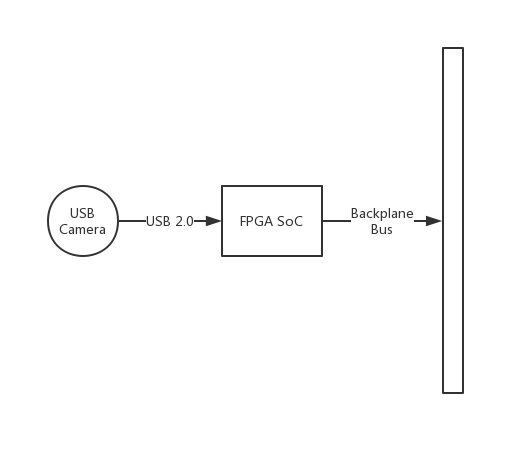
\includegraphics[width=0.7\textwidth]{img/DR00002_Plan1.png}
 \caption{System Diagram for Plan A}	
\end{center}
\end{figure}
\\
\begin{table}[H]
	\centering
		\begin{tabu}{c | c }
		Pro & Con \\ \hline
		Easy for implement & Low Bitrate \\
		Easy to find sensor &  \\
		Come with video encoding &  \\
		\end{tabu}
	\caption{The Pros and Cons Summary}
\end{table}
\newpage
\section{MIPI camera + CrossLink with FPGA chip}
This plan will use a CrossLink chip to translate the MIPI signal to LVDS signal. The FPGA chip will receive the LVDS signal and use internal encoding IP core to process the data and send it out via the backplane bus. The CrossLink and the main chip are both FPGAs. It mean this system can easily increase the number of the camera. Four lane MIPI support up to 4K 180fps frame rate. It also allow future upgrade without change the hardware design due to the flexiblity of FPGA chip.
\begin{figure}[htp]
\begin{center}
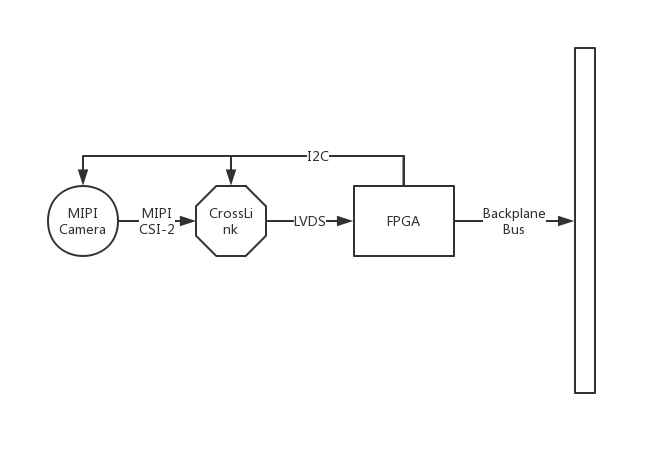
\includegraphics[width=0.7\textwidth]{img/DR00002_Plan2.png}
 \caption{System Diagram for Plan B}	
\end{center}
\end{figure}
\begin{table}[H]
	\centering
		\begin{tabu}{c | c }
		Pro & Con \\ \hline
		Can use any raspberry Pi Camera & Need Encoding Core \\
		High Speed Sensor(Up to 180 FPS) & Hard in PCB design(100$\Omega$ impedance) \\
		Allow futrue upgrade & Long development time \\
		Prevent common mode interference  & Need Extra chip for translation \\
		\end{tabu}
	\caption{The Pros and Cons Summary}
\end{table}
\newpage
\section{LVDS camera with FPGA chip}
This plan will connect a LVDS camera to a FPGA. The FPGA will encode the video and send it via the backplane. The video will be encoded in the FPGA IP core and pack it into the backplane bus packet. Because the camera sensor use the FPGA support standard, it will reduce the problem of format translation. It also allow future upgrade without change the hardware design due to the flexiblity of FPGA chip.
\begin{figure}[htp]
\begin{center}
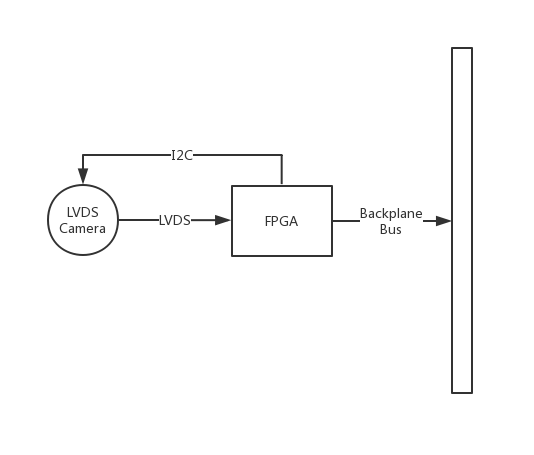
\includegraphics[width=0.7\textwidth]{img/DR00002_Plan3.png}
 \caption{System Diagram for Plan C}	
\end{center}
\end{figure}
\begin{table}[H]
	\centering
		\begin{tabu}{c | c }
		Pro & Con \\ \hline
		Do not need Extra chip for translation & Need Encoding Core \\
		Cheap sensor & Hard in PCB design(100$\Omega$ impedance) \\
		Allow futrue upgrade & Long development time \\
		Prevent common mode interference  &  \\
		\end{tabu}
	\caption{The Pros and Cons Summary}
\end{table}
\newpage
\section{MIPI camera with Multimedia SoC chip}
This plan will use the solution that company provide and add additional chip for the data translation from the USB to backplane bus. Because of the solution mostly will be provided by the company, it will be more stable. However, it lose the ability for upgrade. Also, because it use the MIPI bus, it require the PCB manufacture to use 100$\Omega$ impedance trace to keep the differential pairs stable.
\begin{figure}[htp]
\begin{center}
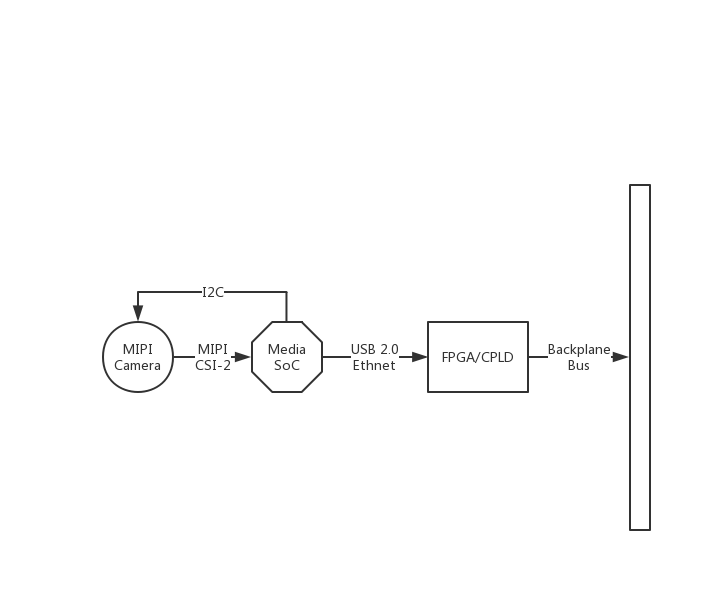
\includegraphics[width=0.7\textwidth]{img/DR00002_Plan4.png}
 \caption{System Diagram for Plan D}	
\end{center}
\end{figure}
\begin{table}[H]
	\centering
		\begin{tabu}{c | c }
		Pro & Con \\ \hline
		Do not need Extra chip for translation & Only support USB 2.0\\
		Cheap sensor & Hard in PCB design(100$\Omega$ impedance) \\
		Do not need Encoding Core & Long development time \\
		Use existing resolution  & \textbf{Need selecting chip} \\
		\end{tabu}
	\caption{The Pros and Cons Summary}
\end{table}
\newpage
\section{MIPI camera with Multimedia DSP and FPGA chip}
This plan use DSP chip as the encoder. However the DSP do not have any video interface, it will need FPGA to finish the format translation and feed it into the DSP chip. Also, because it use the MIPI bus, it require the PCB manufacture to use 100$\Omega$ impedance trace to keep the differential pairs stable. The DSP itself also have a set of SDK need to be take care off. It might require additional time to construct the program.
\begin{figure}[htp]
\begin{center}
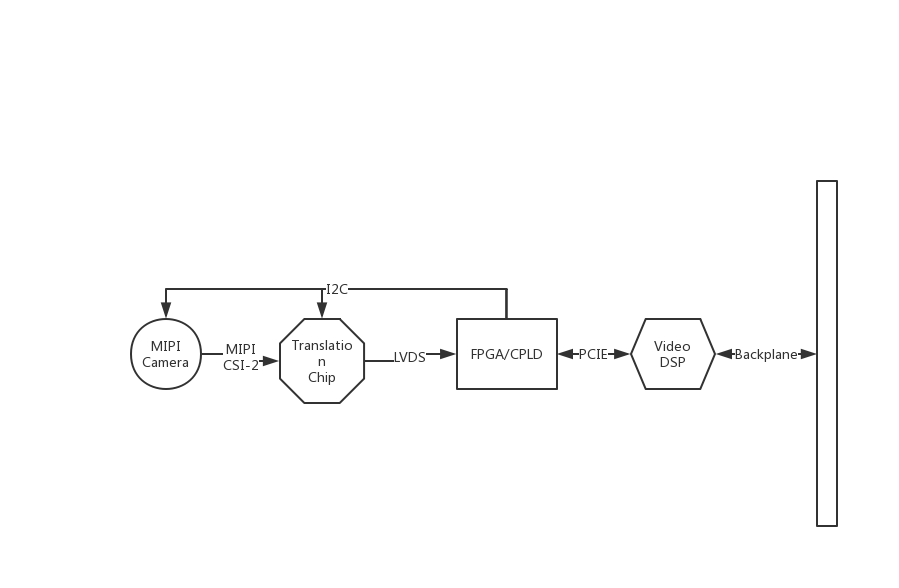
\includegraphics[width=0.7\textwidth]{img/DR00002_Plan5-2.png}
 \caption{System Diagram for Plan F}	
\end{center}
\end{figure}
\begin{table}[H]
	\centering
		\begin{tabu}{c | c }
		Pro & Con \\ \hline
		Do not need Encoding Core & Need extra chip for translation and encoding\\
		Use existing resolution & Hard in PCB design(100$\Omega$ impedance) \\
		 & Long development time \\
		\end{tabu}
	\caption{The Pros and Cons Summary}
\end{table}
\newpage
\chapter{Bibliography}
\printbibliography[heading=none]
%end of document
%**********************************************************************
\end{document}
